%%%%%%%%%%%%%%%%%%%%%%%%%%%%%%%%%%%%%%%%%%%%%%%%%%%%%%%%%%%%%%%%%%%%%%%%
% Escuela Politécnica Superior de la Universidad de Alicante
% Realizado por: Jose Manuel Requena Plens
% Contacto: info@jmrplens.com / Telegram:@jmrplens
%%%%%%%%%%%%%%%%%%%%%%%%%%%%%%%%%%%%%%%%%%%%%%%%%%%%%%%%%%%%%%%%%%%%%%%%

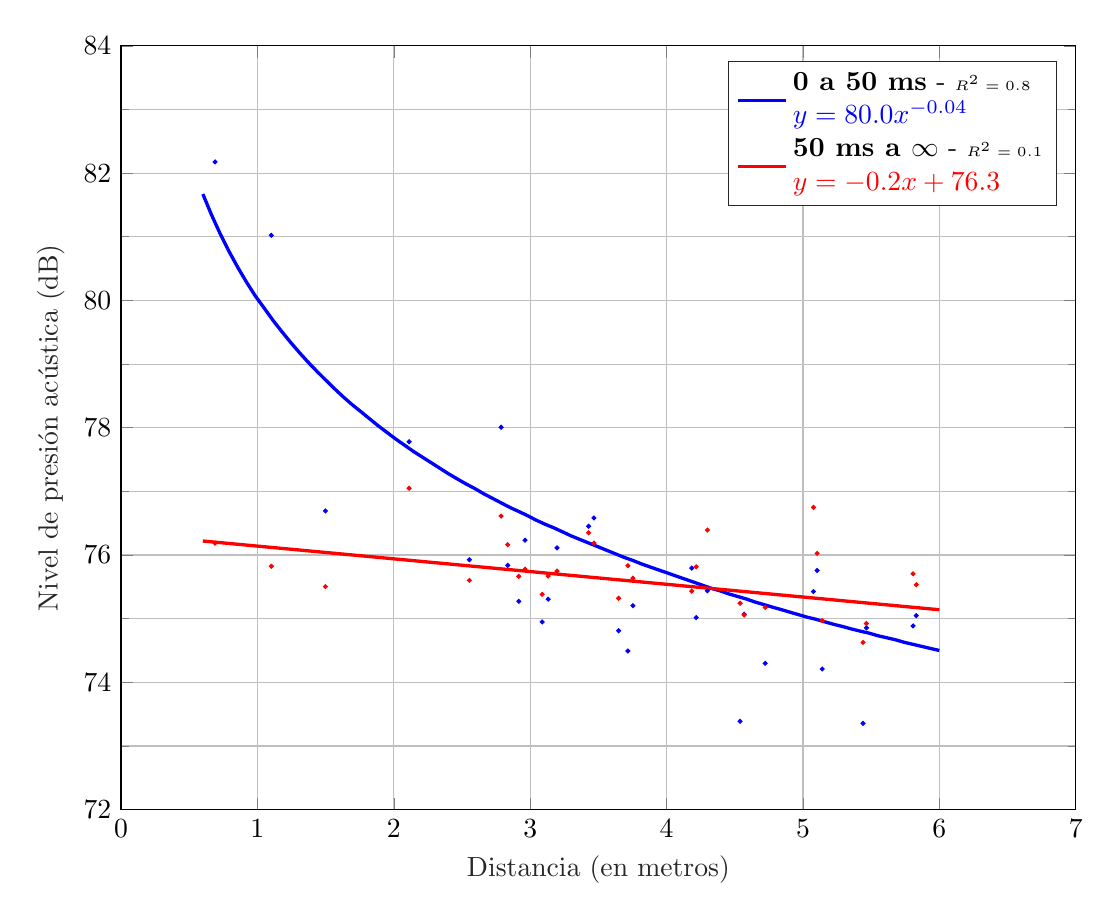
\begin{tikzpicture}

\begin{axis}[%
width=\textwidth,
height=0.8\textwidth,
at={(0\textwidth,0\textwidth)},
scale only axis,
xmin=0,
xmax=7,
xlabel style={font=\color{white!15!black}},
xlabel={Distancia (en metros)},
ymin=72,
ymax=84,
xmajorgrids,
xminorgrids,
ymajorgrids,
yminorgrids,
minor y tick num= 1,
ylabel style={font=\color{white!15!black}},
ylabel={Nivel de presión acústica (dB)},
axis background/.style={fill=white},
legend style={legend cell align=left, align=left, draw=white!15!black}
]
\addplot [color=blue, only marks,mark size=0.7pt, forget plot]
  table[row sep=crcr]{%
0.689492567037533	82.1760231834145\\
1.10208892563169	81.0225435793872\\
1.49833240637717	76.6929736552575\\
2.11248668634857	77.7797341548963\\
2.5540947515705	75.9268678204342\\
2.78664673039121	78.0078667294989\\
2.83511904511963	75.8379926821758\\
2.91626473421053	75.2733361947342\\
2.9626170862938	76.2332705870363\\
3.08787953132891	74.9482250490155\\
3.13169283295792	75.3064321486077\\
3.19677962956473	76.1127065991513\\
3.428206528201	76.4517777633818\\
3.46772259559498	76.5818812618574\\
3.64836949883095	74.8090226514553\\
3.71663826596024	74.4921848339607\\
3.75311870315875	75.2041666937952\\
4.18442349673165	75.7926859018596\\
4.21685902064559	75.0167269886588\\
4.29941856534113	75.4385466917373\\
4.53878838458019	73.3872229047654\\
4.56870878914383	75.0707133021758\\
4.72298634340605	74.2990289518437\\
5.07690850813761	75.4267529690394\\
5.10367514640186	75.757487280947\\
5.14125471067132	74.2096029808742\\
5.44027572830643	73.3546647587015\\
5.46526303118158	74.8548020040326\\
5.80710771382795	74.8859657158564\\
5.83052313261855	75.0478888373477\\
};

\addplot[color=blue,domain=0.6:6, samples=85,line width=1.2]{80.02*x^(-0.04)};
\addlegendentry{\textbf{0 a 50 ms} - \tiny{$R^2 = 0.8$}\\$\color{blue}y = 80.0·x^{-0.04}$}


\addplot [color=red, only marks,mark size=0.7pt, forget plot]
  table[row sep=crcr]{%
0.689492567037533	76.1860324366908\\
1.10208892563169	75.8228245224521\\
1.49833240637717	75.5036949938464\\
2.11248668634857	77.0497144256298\\
2.5540947515705	75.6014044921133\\
2.78664673039121	76.6112713817978\\
2.83511904511963	76.162080733805\\
2.91626473421053	75.6651404039956\\
2.9626170862938	75.7775619322898\\
3.08787953132891	75.3821777509942\\
3.13169283295792	75.6687522168879\\
3.19677962956473	75.7477124982068\\
3.428206528201	76.3485162347617\\
3.46772259559498	76.185858536935\\
3.64836949883095	75.3211330582598\\
3.71663826596024	75.8324897336812\\
3.75311870315875	75.6357978606202\\
4.18442349673165	75.4316552399674\\
4.21685902064559	75.8139630101425\\
4.29941856534113	76.3919969989648\\
4.53878838458019	75.2420141497027\\
4.56870878914383	75.0580538595667\\
4.72298634340605	75.1774090440704\\
5.07690850813761	76.7490410724972\\
5.10367514640186	76.0255133429585\\
5.14125471067132	74.9683820360272\\
5.44027572830643	74.6258521636235\\
5.46526303118158	74.9241893689036\\
5.80710771382795	75.7043411902589\\
5.83052313261855	75.5332426529618\\
};
\addplot[color=red,domain=0.6:6, samples=85,line width=1.2]{-0.2*x+76.34};
\addlegendentry{\textbf{50 ms a $\infty$} - \tiny{$R^2 = 0.1$}\\$\color{red}y = -0.2·x+76.3$}

\end{axis}
\end{tikzpicture}%